%! Author = ruochongli
%! Date = 2023/3/11

% Preamble
\documentclass[./main.tex]{subfiles}

% Packages

% Document
\begin{document}
    \section{Solution}
    We calculated each the coefficient of profit of every facility on every piece of land.
    In Figure~\ref{fig:figureHeapmap}, greener colors means more suitable configuration, and redder colors means less suitable configuration.
    However, color difference between different facilities does not necessarily mean a difference in the coefficient
    of profit between facilities.
    Please see Appendix A for more information about the optimal solution.

    \begin{figure}[H]
        \centering
        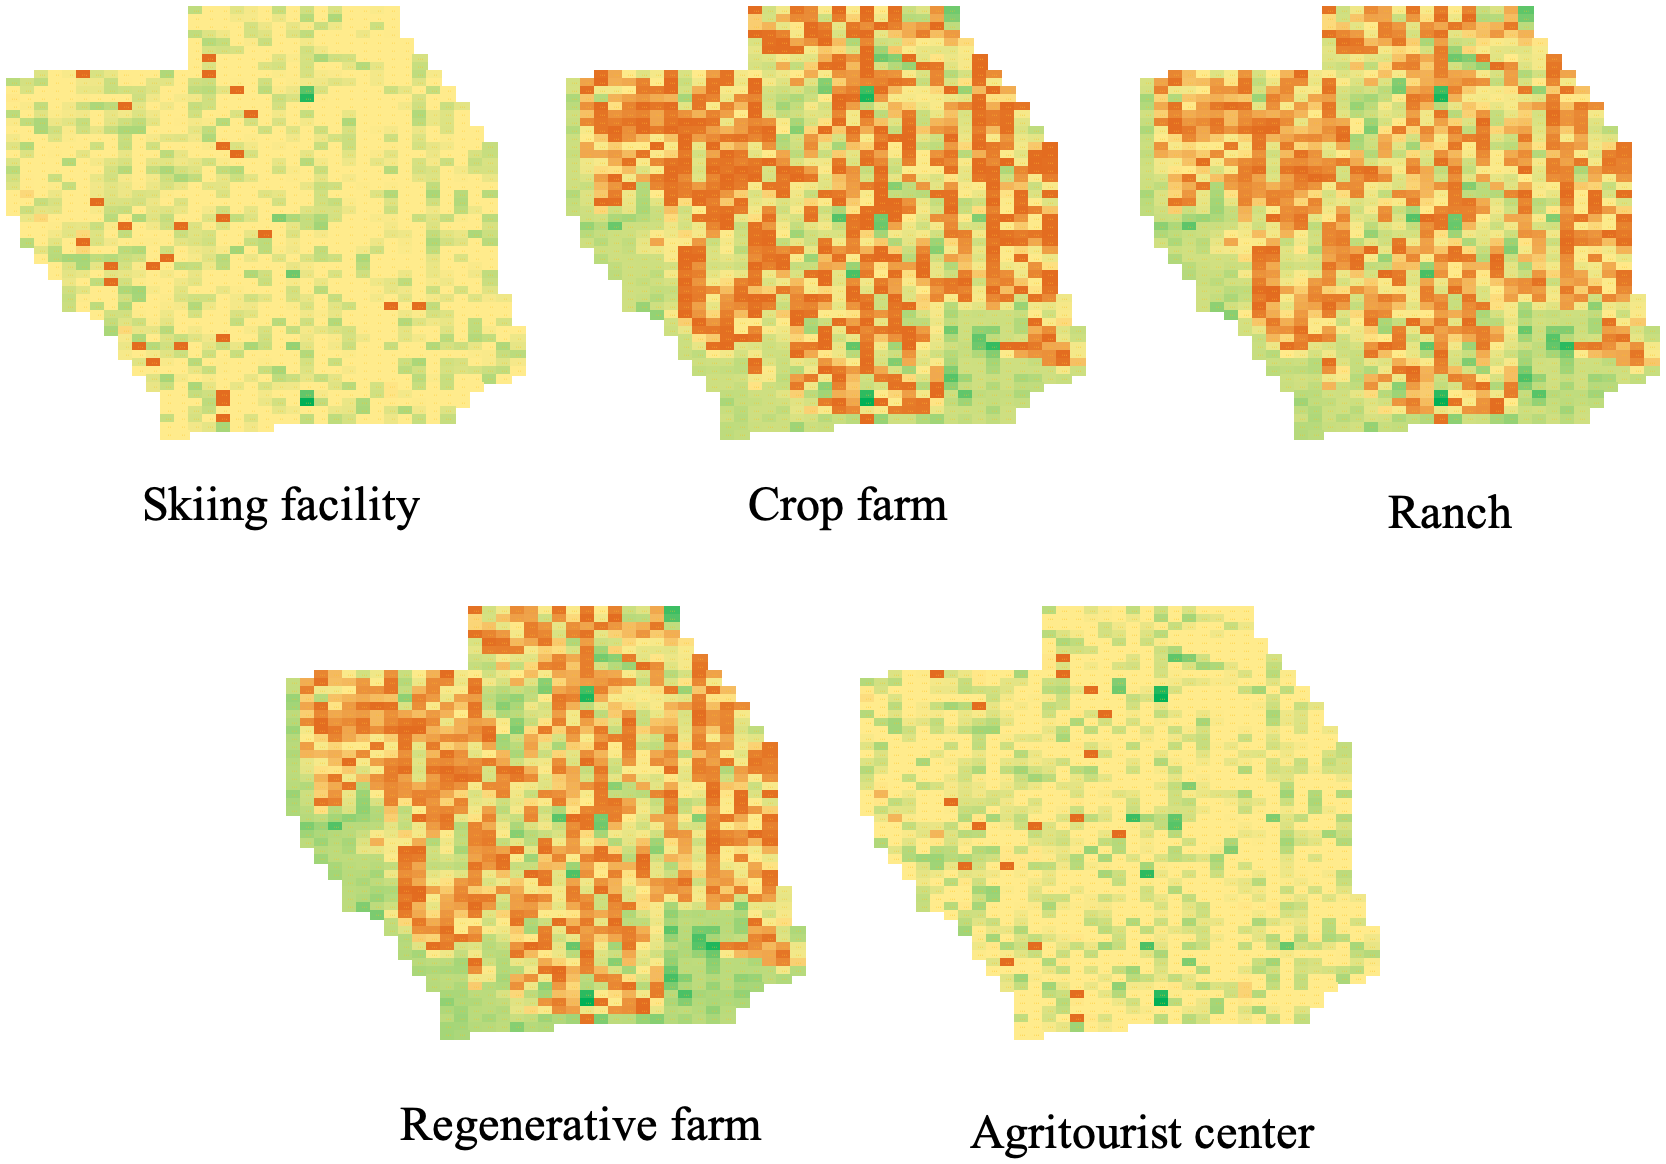
\includegraphics[width=\textwidth]{./figure/figureColored.png}
        \caption{Heatmap of facilities\rq coefficient of profit}
        \label{fig:figureHeapmap}
    \end{figure}





\end{document}